%%%%%%%%%%%%%%%%%%%%%%%%%%%%%%%%%%%%%%%%%%%%%%%%%%%%%%%%%%%%%%%%%
%_____________ ___    _____  __      __ 
%\____    /   |   \  /  _  \/  \    /  \  Institute of Applied
%  /     /    ~    \/  /_\  \   \/\/   /  Psychology
% /     /\    Y    /    |    \        /   Zuercher Hochschule 
%/_______ \___|_  /\____|__  /\__/\  /    fuer Angewandte Wissen.
%        \/     \/         \/      \/                           
%%%%%%%%%%%%%%%%%%%%%%%%%%%%%%%%%%%%%%%%%%%%%%%%%%%%%%%%%%%%%%%%%
%
% Project     : Bachelorarbeit
% Title       : 
% File        : Rev. 00
% Date        : 06.12.2013
% Author      : Till J. Ernst
%
%%%%%%%%%%%%%%%%%%%%%%%%%%%%%%%%%%%%%%%%%%%%%%%%%%%%%%%%%%%%%%%%%
\glsresetall

\let\raggedsection\centering 
\chapter{Grafische Darstellung der Hypothese}\label{chap.appendix_hypotheseGrafisch}
\let\raggedsection\raggedright 
\begin{RaggedRight}
\begin{figure}[ht]
    \centering
    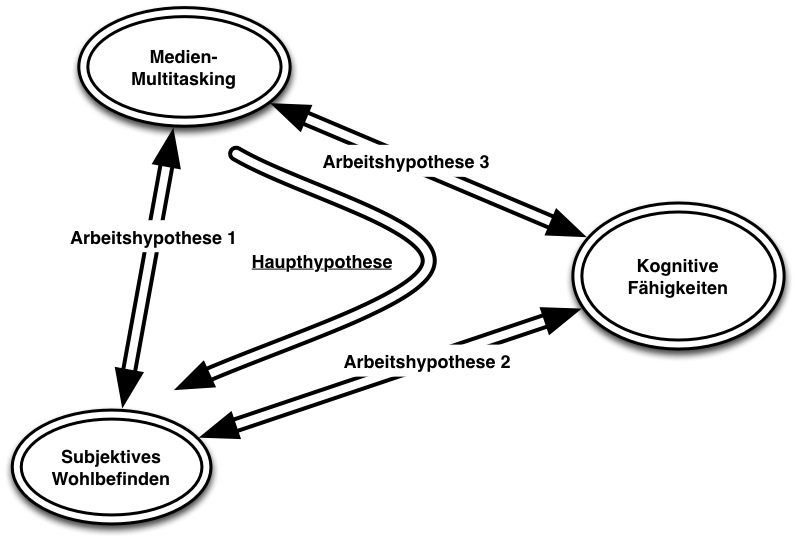
\includegraphics[scale=0.55]{images/grafiken/Hypothesen_Grafisch_v2.pdf}
     \caption{Zusammenhang Hypothesen}
     \label{pic.einleitung.hypothesen}
\end{figure}
\end{RaggedRight}
